\chapter{INTRODUCTION} \label{ch:intro}

\section{Motivation}
  Given the global rise in population, efficient and innovative resource utilization is increasingly important.
Future generations face major challenges regarding food, energy, and water security while addressing major issues associated with global climate change.
Growing concern for the negative environmental impacts of petroleum-based fuel is generating a market for biofuel, especially corn-based ethanol.
However, corn-based ethanol has been heavily criticized for diverting land usage away from food production, for increasing use of fertilizers that impair water quality, and for low return on energy investments for production.
At the same time, a great deal of unutilized saltwater coastline is available for both food and fuel production through seaweed cultivation.
Specifically, the sugar kelp \textit{Saccharina latissima} is known to be a viable source of food,  both for direct human consumption and biofuel production.

%TODO: Nitrogen concerns, wastewater treatment.
Nitrogen leakage into water bodies is a significant ecological problem, and is especially relevant near large conventional agriculture facilities due to run-off from nitrogen-based fertilizers, as well as near wastewater treatment plants.
Waste water treatment plants (WWTPs) in particular are facing increasingly stringent regulation of nutrients in their effluent discharges from the US Environmental Protection Agency (USEPA) and state regulatory agencies.
Nutrient management at WWTPs requires significant infrastructure, operations, and maintenance investments for tertiary treatment processes. Many treatment works are constrained financially or by space limitations in their ability to expand their treatment works.
As an alternative to conventional nutrient remediation techniques, the cultivation of the macroalgae \textit{Saccharina latissima} (sugar kelp) within the nutrient plume of WWTP ocean outfalls has been proposed.
The purpose of such an undertaking would be twofold: to prevent eutrophication of the surrounding ecosystem by sequestering nutrients, and to provide supplemental nutrients that benefit macroalgae cultivation. %TODO: Cite

Large scale macroalgae cultivation has long existed in Eastern Asia due to the popularity of seaweed in Asian cuisine, and low labor costs that facilitate its manual seeding and harvest.
  More recently, less labor-intense and more industrialized kelp aquaculture has been developing in Scandinavia and in the Northeastern United States and Canada.
For example, the MACROSEA project is a four year international research collaboration led by SINTEF, an independent research organization in Norway, and funded by the Research Council of Norway targeting ``successful and predictable production of high quality biomass thereby making significant steps towards industrial macroalgae cultivation in Norway.'' %TODO: Cite this
The project includes both cultivators and scientists, working to develop a precise understanding of the full life cycle of kelp and its interaction with its environment.
A fundamental aspect of this endeavor is the development of mathematical models to describe the growth of kelp.

Recently, a growth model\cite{broch_modelling_2012} for S. latissima has been produced and integrated into the SINMOD\cite{wassmann_modelling_2006} hydrodynamic and ecosystem model of SINTEF.
One aspect of the model which has yet to be fully developed is the availability of light, considering factors such as absorption and scattering by the aquatic medium, as well as by the kelp itself.
This thesis contributes to this effort by developing a first-principles model of the light field in a kelp farming environment.
As a first step, a model for the spatial distribution of kelp is developed.
Radiative transfer theory is then applied to determine the effects of the kelp and water on the availability of light throughout the medium.
A numerical finite difference solution to the Radiative Transfer Equation, followed by asymptotic approximations that prove to be sufficiently accurate and less computationally intensive.
A detailed description of the numerical solution of this model, accompanied by source code for a FORTRAN implementation of the solution.
This model can be used independently, or in conjunction with a kelp growth model to determine the amount of light available for photosynthesis at a single time step.

\begin{figure}[h]
  \centering
  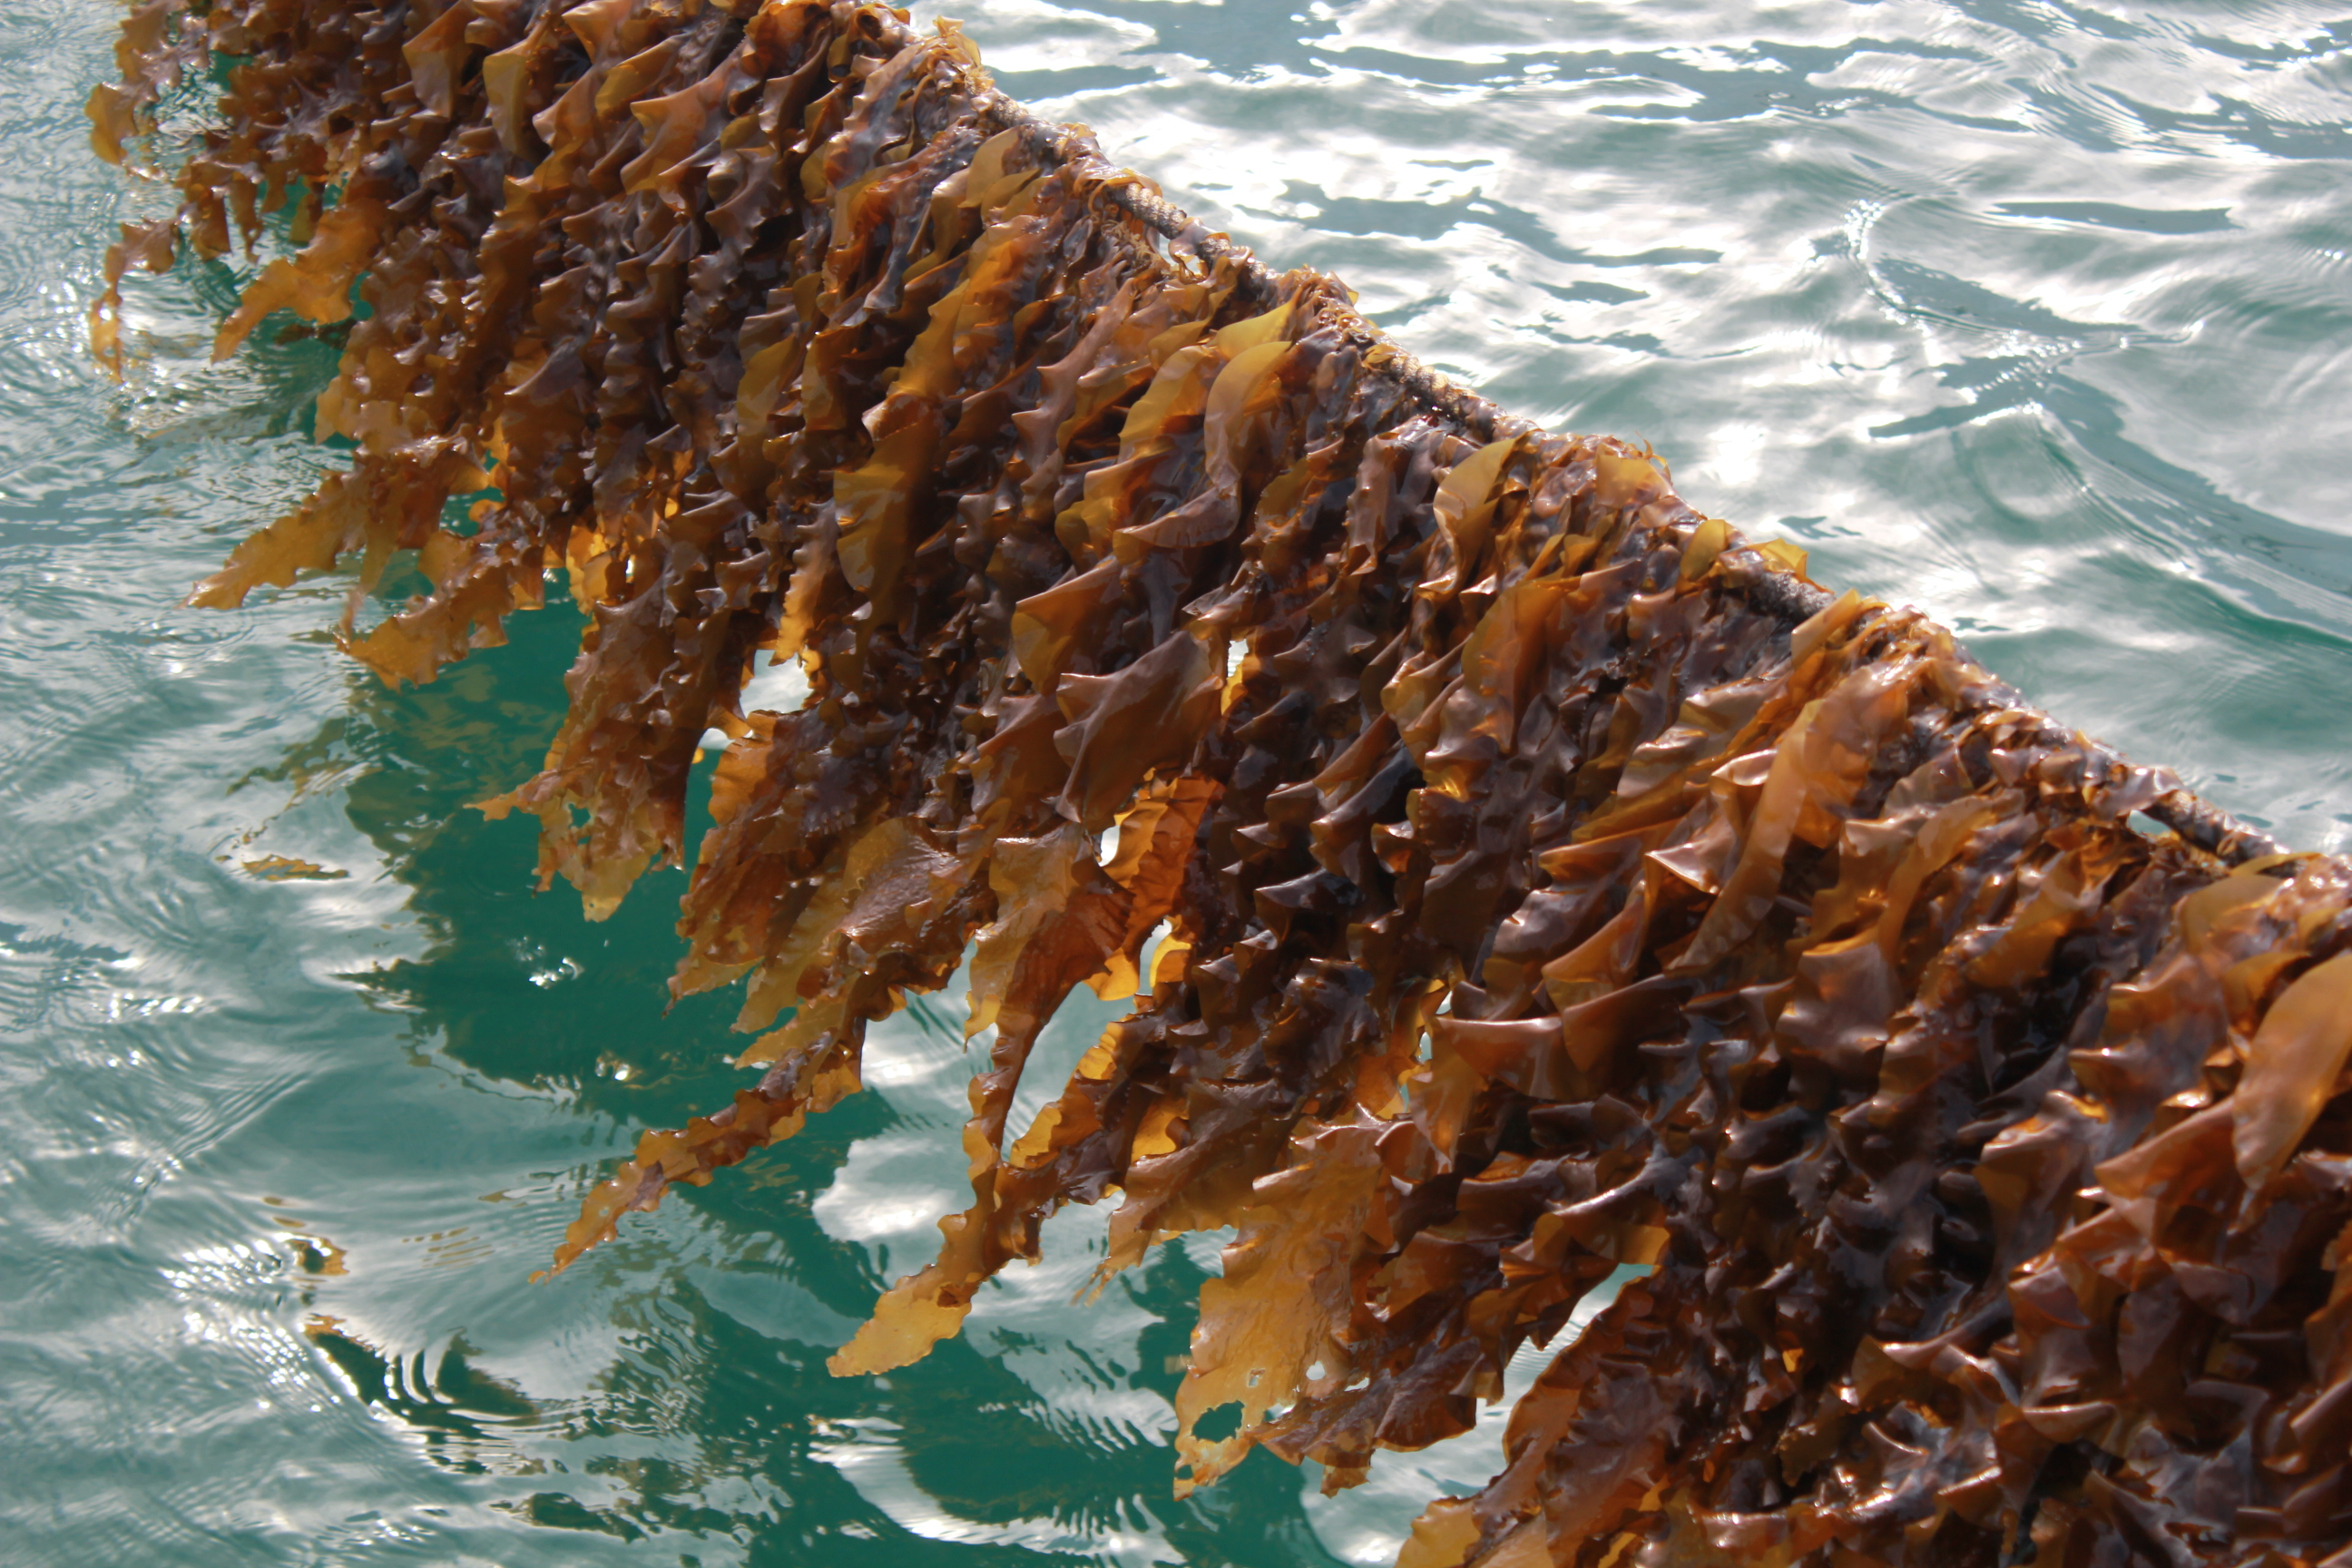
\includegraphics[width=\textwidth]{kelp_photo/kelp_photo1}
  \caption{\textit{Saccharina latissima} being harvested}
  % https://blogs.qub.ac.uk/qubio/files/2016/04/H5-5.jpg
  %TODO: Cite properly or replace with photo from Shane
\end{figure}


\section{Background on Kelp Models}

Mathematical modeling of macroalgae growth is not a new topic, although it is a reemerging one.
Several authors in the second half of the twentieth century were interested in describing the growth and composition of the macroalgae \textit{Macrocystis pyrifera}, commonly known as ``giant kelp,'' which grows prolifically off the coast of southern California.
The first such mathematical model was developed by W.J. North for the Kelp Habitat Improvement Project at the California Institute of Technology in 1968 using seven variables.
By 1974, Nick Anderson greatly expanded on North's work, and created the first comprehensive model of kelp growth which he programmed using FORTRAN\cite{anderson_mathematical_1974}.
In his model, he accounts for solar radiation intensity as a function of time of year and time of day, and refraction on the surface of the water.
He uses a simple model for shading, simply specifying a single parameter which determines the percentage of light that is allowed to pass through the kelp canopy floating on the surface of the water.
He also accounts for attenuation due to turbidity using Beer's Law.
Using this data on the availability of light, he calculates the photosynthesis rates and the growth experienced by the kelp.

Over a decade later in 1987, G.A.
Jackson expanded on Anderson's model for \textit{Macrocystis pyrifera}, with an emphasis on including more environmental parameters and a more complete description of the growth and decay of the kelp\cite{jackson_modelling_1987}. 
The author takes into account respiration, frond decay, and sub-canopy light attenuation due to self-shading.
Light attenuation is represented with a simple exponential model, and self-shading appears as an added term in the decay coefficient.
The author does not consider radial or angular dependence on shading. %TODO:  Check this. Was previously ambiguous.
Jackson also expands Anderson's definition of canopy shading, treating the canopy not as a single layer, but as 0, 1, or 2 discrete layers, each composed of individual fronds.
While this is a significant improvement over Anderson's light model, it is still rather simplistic.

Both Anderson's and Jackson's model were carried out by numerically solving a system of differential equations over small time intervals.
In 1990, M.A. Burgman and V.A. Gerard developed a stochastic population model\cite{burgman_stage-structured_1990}.
This approach is quite different, and functions by dividing kelp plants into groups based on size and age and generating random numbers to determine how the population distribution over these groups changes over time based on measured rates of growth, death, decay, light availability, etc.
In the same year, Nyman et. al. published a similar model alongside a Markov chain model, and compared the results with experimental data collected in New Zealand\cite{nyman_macrocystis_1990}.

In 1996 and 1998 respectively, P. Duarte and J.G. Ferreira used the size-class approach to create a more general model of macroalgae growth, and Yoshimori et. al. created a differential equation model of \textit{Laminaria religiosa} with specific emphasis on temperature dependence of growth rate\cite{duarte_model_1997,yoshimori_mathematical_1998}.
These were the some of the first models of kelp growth that did not specifically relate to \textit{Macrocystis pyrifera} (``giant kelp''). 
Initially, there was a great deal of excitement about this species due to it's incredible size and growth rate, but difficulties in harvesting and negative environmental impacts have caused scientists to investigate other kelp species. % TODO: Cite

\section{Background on Radiative Transfer}
In terms of optical quantities, of primary interest is in the radiance at each point from all directions, which affects the photosynthetic rate of the kelp, and therefore the total amount of biomass producible in a given area as well as the total nutrient remediation potential.
The equation governing the radiance throughout the system is known as the Radiative Transfer Equation (RTE), which has been largely unutilized in the fields of oceanography and aquaculture.
The Radiative Transfer Equation has been used primarily in stellar astrophysics; it's application to marine biology is fairly recent\cite{mobley_radiative_2001}.
In its full form, radiance is a function of 3 spatial dimensions, 2 angular dimensions, and frequency, making for an incredibly complex problem. % TODO: Cite?
In this work, frequency is ignored, only monochromatic radiation is considered.
The RTE states that along a given path, radiance is decreased by absorption and scattering out of the path, while it is increased by emission and scattering into the path.
In our situation, emission is negligible, owing only perhaps to some small luminescent phytoplankton or other anomaly, and can therefore be safely ignored.

% TODO: Remove?
Understanding the growth rate and nutrient recovery by
kelp cultures has important marine biological implications. For example, recent
work by our research group at Clarkson University, the University of Maine, and
SINTEF Fisheries and Aquaculture is investigating kelp aquaculture as a means to
recover nutrients from wastewater effluent plumes in coastal environments into a
valuable biomass feedstock for many products. Current models for kelp growth
place little emphasis on the way in which nearby plants shade one another.
Self-shading may be a significant model feature, though, as light availability
may impact the growth and composition of the kelp biomass, and thus the mixture
of goods that may be derived.

\section{Overview of Thesis}
% TODO: Check for redundancy
The remainder of this document is organized as follows.
In Chapter \ref{chap:kelp}, we develop a probabilistic model to describe the spatial distribution of kelp by assuming simple distributions for the lengths and orientations of fronds.
We begin Chapter \ref{chap:light} with a survey of fundamental radiometric quantities and optical properties of matter.
We use the spatial kelp distribution from Chapter \ref{chap:kelp} to determine optical properties of the combined water-kelp medium.
We then present the Radiative Transfer Equation, an integro-partial differential equation which describes the the light field as a function of position and angle.
An asymptotic expansion is explored for cases where absorption dominates scattering in the medium, such as in very clear water or high kelp density.
In Chapter \ref{chap:numerical}, details are given for the numerical solution of the equations from Chapters \ref{chap:kelp} and \ref{chap:light}.
Both the full finite difference solution and the asymptotic approximation are described.
Next, in Chapter \ref{chap:parameters}, we discuss the availability of necessary parameters in the literature.
For those which are not readily available, we give rough estimates and briefly describe experimental methods for their determination.
Then, in Chapter \ref{chap:model_analysis}, we investigate the necessary grid resolution for adequate accuracy in the full finite difference solution and compare to the asymptotic approximation for a few parameter sets.
Further, we determine the effect of varying a few key parameters on the light field predicted by the asymptotic approximation.
Afterwards, the light model developed here is used in a numerical simulation of kelp growth, and the predicted light field and biomass production are compared to those predicted by a simpler 1D exponential decay light model.
Finally, we conclude with Chapter \ref{chap:conclusion} by giving a brief summary of the model, discuss and its performance, and suggest improvements and avenues for future work.
